% This LaTeX was auto-generated from MATLAB code.
% To make changes, update the MATLAB code and export to LaTeX again.

\documentclass{article}

\usepackage[utf8]{inputenc}
\usepackage[T1]{fontenc}
\usepackage{lmodern}
\usepackage{graphicx}
\usepackage{color}
\usepackage{hyperref}
\usepackage{amsmath}
\usepackage{amsfonts}
\usepackage{epstopdf}
\usepackage[table]{xcolor}
\usepackage{matlab}
\usepackage[paperheight=795pt,paperwidth=614pt,top=72pt,bottom=72pt,right=72pt,left=72pt,heightrounded]{geometry}

\sloppy
\epstopdfsetup{outdir=./}
\graphicspath{ {./LIVE_SCRIPT_media/} }

\begin{document}

\matlabtitle{Pellet Smoker: Model B}


\matlabheading{Set Particulars}

\begin{matlabcode}
p.C_f = 500;
p.k_f = 150;
p.k_ca = 25;
p.C_c = 2500;
p.k_fa = 20;
p.gamma = 1000;
p.T_amb = 25;
p.u_p_max = 10;
p.u_p_min = 0;
p.u_f_max = 1;
p.u_f_min = 0;
if false % uncertainty in model
    sigma = 0.20;
    p.C_f = 500*(1 + sigma * randn);
    p.k_f = 150*(1 + sigma * randn);
    p.k_ca = 25*(1 + sigma * randn);
    p.C_c = 2500*(1 + sigma * randn);
    p.k_fa = 20*(1 + sigma * randn);
    p.gamma = 1000*(1 + sigma * randn);
    p.T_amb = 25*(1 + sigma * randn);
end
\end{matlabcode}
\begin{matlaboutput}
u = 2x1329
         0    0.2534    0.4859    0.7003    0.8991    1.0844    1.2575    1.4199    1.5733    1.7854    1.9850    2.1732    2.3514    2.6034    2.8363    3.0511    3.2498    3.5065    3.7340    3.9333    4.1077    4.3071    4.4670    4.5903    4.6831    4.7679    4.8123    4.8184    4.8034    4.8435    4.8013    4.5998    4.4645    4.5107    4.5053    4.4147    4.3389    4.3480    4.3316    4.2720    4.2219    4.2333    4.2196    4.1511    4.1016    4.1750    4.1876    4.0618    3.9854    4.1444
         0    0.1689    0.3240    0.4669    0.5994    0.7229    0.8384    0.9466    1.0000    1.0000    1.0000    1.0000    1.0000    1.0000    1.0000    1.0000    1.0000    1.0000    1.0000    1.0000    1.0000    1.0000    1.0000    1.0000    1.0000    1.0000    1.0000    1.0000    1.0000    1.0000    1.0000    1.0000    1.0000    1.0000    1.0000    1.0000    1.0000    1.0000    1.0000    1.0000    1.0000    1.0000    1.0000    1.0000    1.0000    1.0000    1.0000    1.0000    1.0000    1.0000

\end{matlaboutput}
\begin{center}
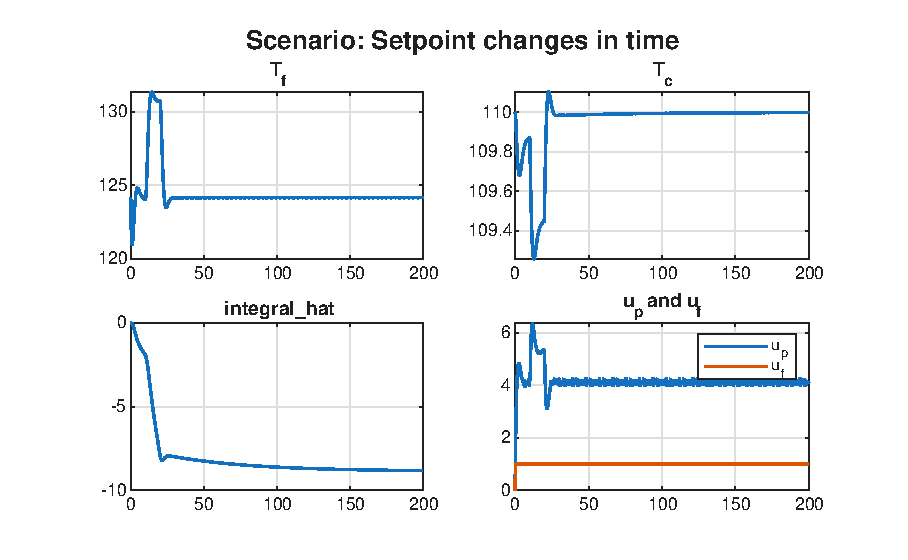
\includegraphics[width=\maxwidth{56.196688409433015em}]{figure_0.eps}
\end{center}


\matlabheading{Integral Action}

\begin{matlabcode}
% initialization points
init_points.T_c_start = p.T_amb;
init_points.m_p_start = 10000;
% linearization and timeseries
lin_timeseries.t_min = 0;
lin_timeseries.t_max = 120;
lin_timeseries.lin = linearize(p, [0.4; 0.6]);
T_c_set_series = @(t) (t<=30)*p.T_amb+(t>30&&t<=600)*110+(t>1200)*130;
lin_timeseries.setpoint = @(t) [Tce2Tfe(p,T_c_set_series(t)); T_c_set_series(t); 0];
lin_timeseries.door_status = @(t) (t>=50)&&(t<20);

% Comparative simulations on integral action
[basic.t, basic.x_aug, basic.u] = run_simulation(p, init_points, lin_timeseries, @basic_observer, @basic_feedback);
[int.t, int.x_aug, int.u] = run_simulation(p, init_points, lin_timeseries, @integral_observer, @integral_feedback);
[sat.t, sat.x_aug, sat.u] = run_simulation(p, init_points, lin_timeseries, @saturating_integral_observer, @integral_feedback);

figure;
plot(basic.t, basic.x_aug(2,:), 'LineWidth', 1.5); hold on;
xlabel('Time [s]');
ylabel(['T_c [' char(176) 'C]']);
title('Observer Feedback with no Integral Action');
grid on;
xline(30,  '--k', ['T_c\_set=110' char(176) 'C]'],  'LabelHorizontalAlignment','right');
\end{matlabcode}
\begin{center}
\includegraphics[width=\maxwidth{40.14049172102359em}]{figure_1.png}
\end{center}
\begin{matlabcode}

% plot
figure;
title("Anti-Windup Integral Action vs Saturating Integral Action")
subplot(2,1,1);
plot(int.t,   int.x_aug(2,:),   'LineWidth', 1.5); hold on;
plot(sat.t,   sat.x_aug(2,:),   'LineWidth', 1.5);
xline(30,  '--k', ['T_c\_set=110' char(176) 'C'],  'LabelHorizontalAlignment','right');
hold off;
xlabel('Time [s]');
ylabel(['T_c [' char(176) 'C']);
title('T_c Comparison');
legend('integral', 'saturating integral');
grid on;
subplot(2,1,2);
plot(int.t, int.x_aug(7,:), 'LineWidth', 1.5); hold on;
plot(sat.t, sat.x_aug(7,:), 'LineWidth', 1.5);
hold off;
xlabel('Time [s]');
ylabel('integral\_hat');
title('Integral Observer Comparison');
legend('integral', 'saturating integral');
grid on;
\end{matlabcode}
\begin{center}
\includegraphics[width=\maxwidth{40.14049172102359em}]{figure_2.png}
\end{center}


\matlabheading{Disturbance Rejection}

\begin{matlabcode}
% initialization points
t_min = 0;
t_max = 200;
T_c_start = 110;
T_c_set = 110; % static setpoint. series setpoint also defined below
m_p_start = 10000;

% linearization and timeseries
lin = linearize(p, [0.4; 0.6]);
T_c_set_series = @(t) (t<=600)*110+(t>600&&t<1200)*110+(t>1200)*130;
setpoint = @(t) [Tce2Tfe(p,T_c_set_series(t)); T_c_set_series(t); 0];
door_status = @(t) (t>=10)&&(t<20);

% set up x_aug_0
x_0 = [Tce2Tfe(p, T_c_start); T_c_start; m_p_start];
x_hat_0 = [Tce2Tfe(p, T_c_start); T_c_start; m_p_start];
integral_hat_0 = 0;
u_hat_0 = [0; 0];
% definition
x_aug_0 = [x_0; x_hat_0; integral_hat_0];% u_hat_0];

% differential equation
x_dot_aug = @(t,x) full_differential_equation(x, @nonlinear_model, @saturating_integral_observer, @integral_feedback, setpoint(t), door_status(t), lin, p);

% use ode45 to solve differential equation
[t, result] = ode45(x_dot_aug, [t_min; t_max], x_aug_0);
result = result'; % get the results as column vector

% recover your u timeseries from x_hat
u = recover_u(@integral_feedback, linspace(t_min,t_max,size(result,2)), result(4:6,:), result(7,:), setpoint, p, lin)

%x_hat, integral_hat, setpoint, p, lin

% plot!
plot_all(t, result, u, "Disturbance Rejection")
\end{matlabcode}


\matlabheading{Profile Tracking}

\begin{matlabcode}
% initialization points
init_points.T_c_start = p.T_amb;
init_points.m_p_start = 10000;
% linearization and timeseries
lin_timeseries.t_min = 0;
lin_timeseries.t_max = 1800;
lin_timeseries.lin = linearize(p, [0.4; 0.6]);
T_c_set_series = @(t) (t<=600)*90+((t>600).*(t<=1200))*110+(t>1200)*130;
lin_timeseries.setpoint = @(t) [Tce2Tfe(p,T_c_set_series(t)); T_c_set_series(t); 0];
lin_timeseries.door_status = @(t) 0 % never
\end{matlabcode}
\begin{matlaboutput}
lin_timeseries = struct with fields:
             t_min: 0
             t_max: 1800
               lin: [1x1 struct]
    T_c_set_series: @(t)(t<=300)*p.T_amb+(t>60&&t<=120)*110+(t>1200)*130
          setpoint: @(t)[Tce2Tfe(p,T_c_set_series(t));T_c_set_series(t);0]
       door_status: @(t)0

\end{matlaboutput}
\begin{matlabcode}

% Comparative simulations on integral action
[sat.t, sat.x_aug, sat.u] = run_simulation(p, init_points, lin_timeseries, @saturating_integral_observer, @integral_feedback);

% plot
figure;
sgtitle("Profile Tracking (Saturating Integral)")
subplot(2,1,1);
plot(sat.t,   sat.x_aug(2,:),   'LineWidth', 1.5); hold on;
set = T_c_set_series(sat.t);
h2 = plot(sat.t,set,   'LineWidth', 1.5, 'LineStyle', ':');
uistack(h2, 'bottom');
legend('profile setpoint', 'T_c')
hold off;
xlabel('Time [s]');
ylabel(['T_c [' char(176) 'C']);
title('T_c vs. profile');
yticks([10 50 90 130]);
xlim([0 1800])
grid on;
subplot(2,1,2);
plot(sat.t, sat.u(1,:), 'LineWidth', 1.2); hold on;
plot(sat.t, sat.u(2,:), 'LineWidth', 1.2);
title('u_p and u_f');
legend('u_p','u_f');
xlim([0 1800])
grid on;
\end{matlabcode}
\begin{center}
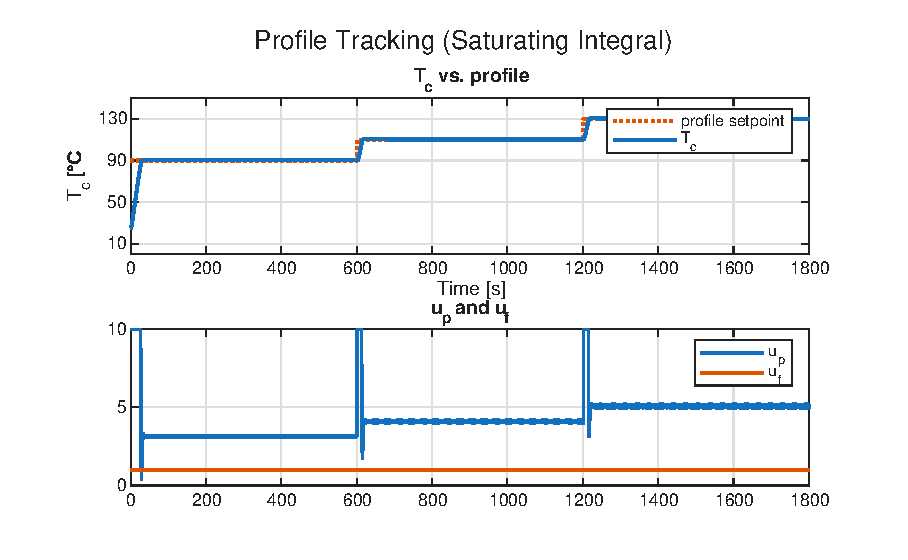
\includegraphics[width=\maxwidth{56.196688409433015em}]{figure_3.eps}
\end{center}
\begin{matlaboutput}
lin_timeseries = struct with fields:
             t_min: 0
             t_max: 1800
               lin: [1x1 struct]
    T_c_set_series: @(t)(t<=300)*p.T_amb+(t>60&&t<=120)*110+(t>1200)*130
          setpoint: @(t)[Tce2Tfe(p,T_c_set_series(t));T_c_set_series(t);0]
       door_status: @(t)0

lin_timeseries = struct with fields:
             t_min: 0
             t_max: 1800
               lin: [1x1 struct]
    T_c_set_series: @(t)(t<=300)*p.T_amb+(t>60&&t<=120)*110+(t>1200)*130
          setpoint: @(t)[Tce2Tfe(p,T_c_set_series(t));T_c_set_series(t);0]
       door_status: @(t)0

lin_timeseries = struct with fields:
             t_min: 0
             t_max: 1800
               lin: [1x1 struct]
    T_c_set_series: @(t)(t<=300)*p.T_amb+(t>60&&t<=120)*110+(t>1200)*130
          setpoint: @(t)[Tce2Tfe(p,T_c_set_series(t));T_c_set_series(t);0]
       door_status: @(t)0

lin_timeseries = struct with fields:
             t_min: 0
             t_max: 1800
               lin: [1x1 struct]
    T_c_set_series: @(t)(t<=300)*p.T_amb+(t>60&&t<=120)*110+(t>1200)*130
          setpoint: @(t)[Tce2Tfe(p,T_c_set_series(t));T_c_set_series(t);0]
       door_status: @(t)0

lin_timeseries = struct with fields:
             t_min: 0
             t_max: 1800
               lin: [1x1 struct]
    T_c_set_series: @(t)(t<=300)*p.T_amb+(t>60&&t<=120)*110+(t>1200)*130
          setpoint: @(t)[Tce2Tfe(p,T_c_set_series(t));T_c_set_series(t);0]
       door_status: @(t)0

lin_timeseries = struct with fields:
             t_min: 0
             t_max: 1800
               lin: [1x1 struct]
    T_c_set_series: @(t)(t<=300)*p.T_amb+(t>60&&t<=120)*110+(t>1200)*130
          setpoint: @(t)[Tce2Tfe(p,T_c_set_series(t));T_c_set_series(t);0]
       door_status: @(t)0

lin_timeseries = struct with fields:
             t_min: 0
             t_max: 1800
               lin: [1x1 struct]
    T_c_set_series: @(t)(t<=300)*p.T_amb+(t>60&&t<=120)*110+(t>1200)*130
          setpoint: @(t)[Tce2Tfe(p,T_c_set_series(t));T_c_set_series(t);0]
       door_status: @(t)0

lin_timeseries = struct with fields:
             t_min: 0
             t_max: 1800
               lin: [1x1 struct]
    T_c_set_series: @(t)(t<=300)*p.T_amb+(t>60&&t<=120)*110+(t>1200)*130
          setpoint: @(t)[Tce2Tfe(p,T_c_set_series(t));T_c_set_series(t);0]
       door_status: @(t)0

lin_timeseries = struct with fields:
             t_min: 0
             t_max: 1800
               lin: [1x1 struct]
    T_c_set_series: @(t)(t<=300)*p.T_amb+(t>60&&t<=120)*110+(t>1200)*130
          setpoint: @(t)[Tce2Tfe(p,T_c_set_series(t));T_c_set_series(t);0]
       door_status: @(t)0

lin_timeseries = struct with fields:
             t_min: 0
             t_max: 1800
               lin: [1x1 struct]
    T_c_set_series: @(t)(t<=300)*p.T_amb+(t>60&&t<=120)*110+(t>1200)*130
          setpoint: @(t)[Tce2Tfe(p,T_c_set_series(t));T_c_set_series(t);0]
       door_status: @(t)0

lin_timeseries = struct with fields:
             t_min: 0
             t_max: 1800
               lin: [1x1 struct]
    T_c_set_series: @(t)(t<=300)*p.T_amb+(t>60&&t<=120)*110+(t>1200)*130
          setpoint: @(t)[Tce2Tfe(p,T_c_set_series(t));T_c_set_series(t);0]
       door_status: @(t)0

lin_timeseries = struct with fields:
             t_min: 0
             t_max: 1800
               lin: [1x1 struct]
    T_c_set_series: @(t)(t<=300)*p.T_amb+(t>60&&t<=120)*110+(t>1200)*130
          setpoint: @(t)[Tce2Tfe(p,T_c_set_series(t));T_c_set_series(t);0]
       door_status: @(t)0

lin_timeseries = struct with fields:
             t_min: 0
             t_max: 1800
               lin: [1x1 struct]
    T_c_set_series: @(t)(t<=300)*p.T_amb+(t>60&&t<=120)*110+(t>1200)*130
          setpoint: @(t)[Tce2Tfe(p,T_c_set_series(t));T_c_set_series(t);0]
       door_status: @(t)0

lin_timeseries = struct with fields:
             t_min: 0
             t_max: 1800
               lin: [1x1 struct]
    T_c_set_series: @(t)(t<=300)*p.T_amb+(t>60&&t<=120)*110+(t>1200)*130
          setpoint: @(t)[Tce2Tfe(p,T_c_set_series(t));T_c_set_series(t);0]
       door_status: @(t)0

lin_timeseries = struct with fields:
             t_min: 0
             t_max: 1800
               lin: [1x1 struct]
    T_c_set_series: @(t)(t<=300)*p.T_amb+(t>60&&t<=120)*110+(t>1200)*130
          setpoint: @(t)[Tce2Tfe(p,T_c_set_series(t));T_c_set_series(t);0]
       door_status: @(t)0

lin_timeseries = struct with fields:
             t_min: 0
             t_max: 1800
               lin: [1x1 struct]
    T_c_set_series: @(t)(t<=300)*p.T_amb+(t>60&&t<=120)*110+(t>1200)*130
          setpoint: @(t)[Tce2Tfe(p,T_c_set_series(t));T_c_set_series(t);0]
       door_status: @(t)0

lin_timeseries = struct with fields:
             t_min: 0
             t_max: 1800
               lin: [1x1 struct]
    T_c_set_series: @(t)(t<=300)*p.T_amb+(t>60&&t<=120)*110+(t>1200)*130
          setpoint: @(t)[Tce2Tfe(p,T_c_set_series(t));T_c_set_series(t);0]
       door_status: @(t)0

lin_timeseries = struct with fields:
             t_min: 0
             t_max: 1800
               lin: [1x1 struct]
    T_c_set_series: @(t)(t<=300)*p.T_amb+(t>60&&t<=120)*110+(t>1200)*130
          setpoint: @(t)[Tce2Tfe(p,T_c_set_series(t));T_c_set_series(t);0]
       door_status: @(t)0

lin_timeseries = struct with fields:
             t_min: 0
             t_max: 1800
               lin: [1x1 struct]
    T_c_set_series: @(t)(t<=300)*p.T_amb+(t>60&&t<=120)*110+(t>1200)*130
          setpoint: @(t)[Tce2Tfe(p,T_c_set_series(t));T_c_set_series(t);0]
       door_status: @(t)0

lin_timeseries = struct with fields:
             t_min: 0
             t_max: 1800
               lin: [1x1 struct]
    T_c_set_series: @(t)(t<=300)*p.T_amb+(t>60&&t<=120)*110+(t>1200)*130
          setpoint: @(t)[Tce2Tfe(p,T_c_set_series(t));T_c_set_series(t);0]
       door_status: @(t)0

\end{matlaboutput}
\begin{center}
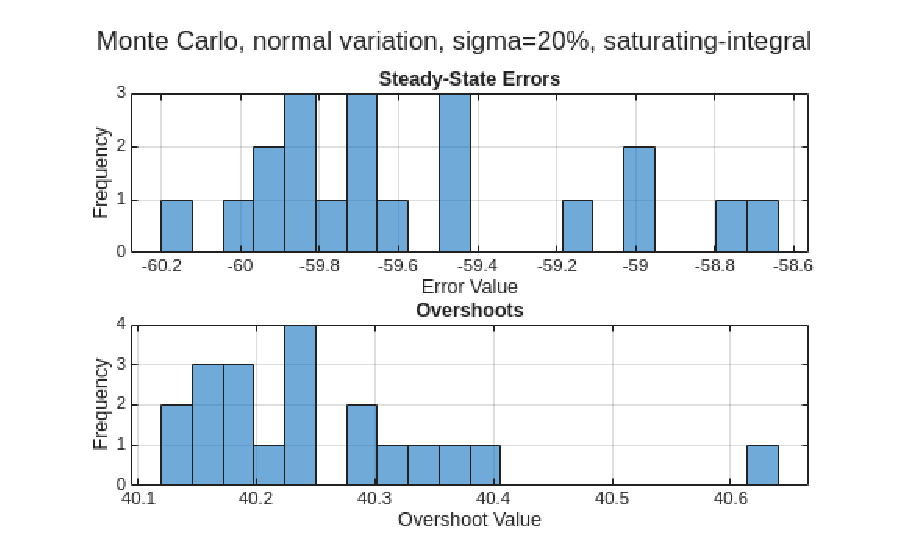
\includegraphics[width=\maxwidth{56.196688409433015em}]{figure_4.eps}
\end{center}


\vspace{1em}

\end{document}
